\subsubsection{Estimation de la matrice P}

Pour modéliser la séquence d'ADN fournie (\texttt{seq1}) sous forme de chaîne de Markov, 
nous devons estimer sa matrice de transition $P$. Les états de la chaîne correspondent aux 
quatre nucléotides, numérotés de 1 à 4 : A (1), C (2), G (3), et T (4).

La probabilité de transition de l'état $i$ vers l'état $j$, notée $P_{i,j}$, 
s'estime par la méthode du maximum de vraisemblance (MLE). 
Cet estimateur correspond à la fréquence empirique des transitions 
observées dans la séquence :

\begin{equation}
    \hat{P}_{i,j} = \frac{N_{i,j}}{\sum_{k=1}^{4} N_{i,k}}
\end{equation}
où $N_{i,j}$ représente le nombre de fois où le nucléotide $i$ est immédiatement 
suivi du nucléotide $j$ dans \texttt{seq1}.

En appliquant cette formule sur notre séquence, nous obtenons la 
matrice de transition empirique suivante (arrondie à 3 décimales) :

\begin{equation}
    P = 
    \begin{pmatrix}
        P_{AA} & P_{AC} & P_{AG} & P_{AT} \\
        P_{CA} & P_{CC} & P_{CG} & P_{CT} \\
        P_{GA} & P_{GC} & P_{GG} & P_{GT} \\
        P_{TA} & P_{TC} & P_{TG} & P_{TT}
    \end{pmatrix}
    =
    \begin{pmatrix}
        0.097 & 0.505 & 0.278 & 0.120 \\ % Row A
        0.253 & 0.246 & 0.262 & 0.239 \\ % Row C
        0.311 & 0.493 & 0.108 & 0.089 \\ % Row G
        0.696 & 0.098 & 0.098 & 0.108    % Row T
    \end{pmatrix}
\end{equation}

\subparagraph{Diagramme d'états}
Le graphe orienté ci-dessous illustre la dynamique de cette chaîne de Markov. 
Les nœuds représentent les états (A, C, G, T) et les arêtes indiquent les probabilités 
de transition $\hat{P}_{i,j}$.

\begin{figure}[ht]
    \centering
    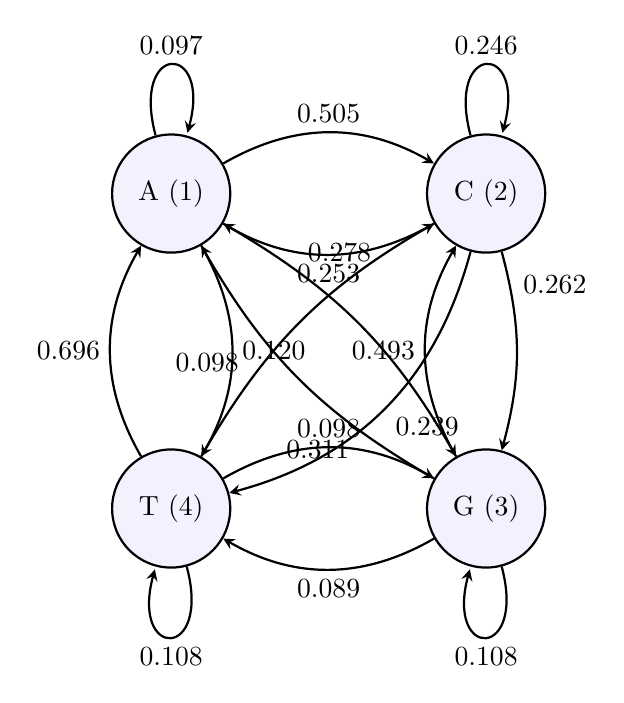
\begin{tikzpicture}[->, >=stealth, node distance=4cm, auto, thick, state/.style={circle, draw, minimum size=1.5cm, fill=blue!5}]
        % Nœuds
        \node[state] (A) {A (1)};
        \node[state, right of=A] (C) {C (2)};
        \node[state, below of=A] (T) {T (4)};
        \node[state, right of=T] (G) {G (3)};

        % Transitions depuis A (Row 1)
        \path (A) edge[loop above] node {0.097} (A)
              (A) edge[bend left] node {0.505} (C)
              (A) edge[bend left=15] node[near start] {0.278} (G)
              (A) edge[bend left] node {0.120} (T);

        % Transitions depuis C (Row 2)
        \path (C) edge[loop above] node {0.246} (C)
              (C) edge[bend left] node {0.253} (A)
              (C) edge[bend left] node {0.239} (T)
              (C) edge[bend left=15] node[near start] {0.262} (G);

        % Transitions depuis G (Row 3)
        \path (G) edge[loop below] node {0.108} (G)
              (G) edge[bend left] node {0.493} (C)
              (G) edge[bend left=15] node[near start] {0.311} (A)
              (G) edge[bend left] node {0.089} (T);

        % Transitions depuis T (Row 4)
        \path (T) edge[loop below] node {0.108} (T)
              (T) edge[bend left] node {0.696} (A)
              (T) edge[bend left=15] node[near start] {0.098} (C)
              (T) edge[bend left] node {0.098} (G);
    \end{tikzpicture}
    \caption{Diagramme d'états de la chaîne de Markov modélisant \texttt{seq1}.}
    \label{fig:markov_seq1}
\end{figure}